\providecolor{stewartcyan}{RGB}{0, 136, 175}
\providecolor{stewartred}{RGB}{208, 40, 36}

\fancyhead[LE]{\fontsize{8.5pt}{10pt}\selectfont\textbf{\textsf{\thepage}}\quad \textbf{\textsf{CHƯƠNG 1}}\quad \textsf{Các hàm số và Mô hình}}
\fancyhead[RO]{\fontsize{8.5pt}{10pt}\selectfont\textsf{MỤC 1.5}\quad \textbf{\textsf{\thepage}}}

\noindent
\begin{minipage}[t]{0.265\textwidth}
    \fontsize{8pt}{10pt}\selectfont
    \vspace*{0pt}
    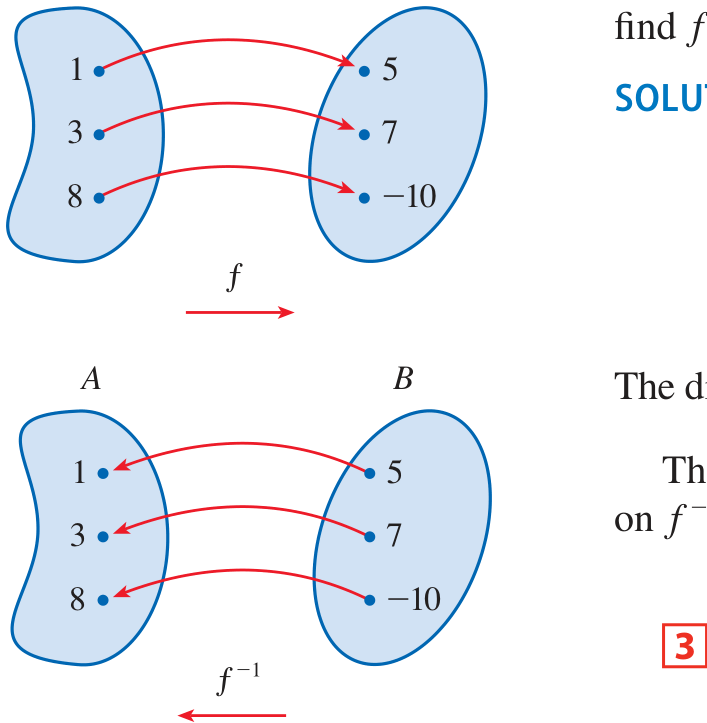
\includegraphics[width=0.92\linewidth]{images/p0091_fig6.png}
    \vspace{3pt}

    \textbf{\textsf{HÌNH 6}}\\
    Hàm ngược đảo ngược các đầu vào và đầu ra.

    \vspace{65pt}
    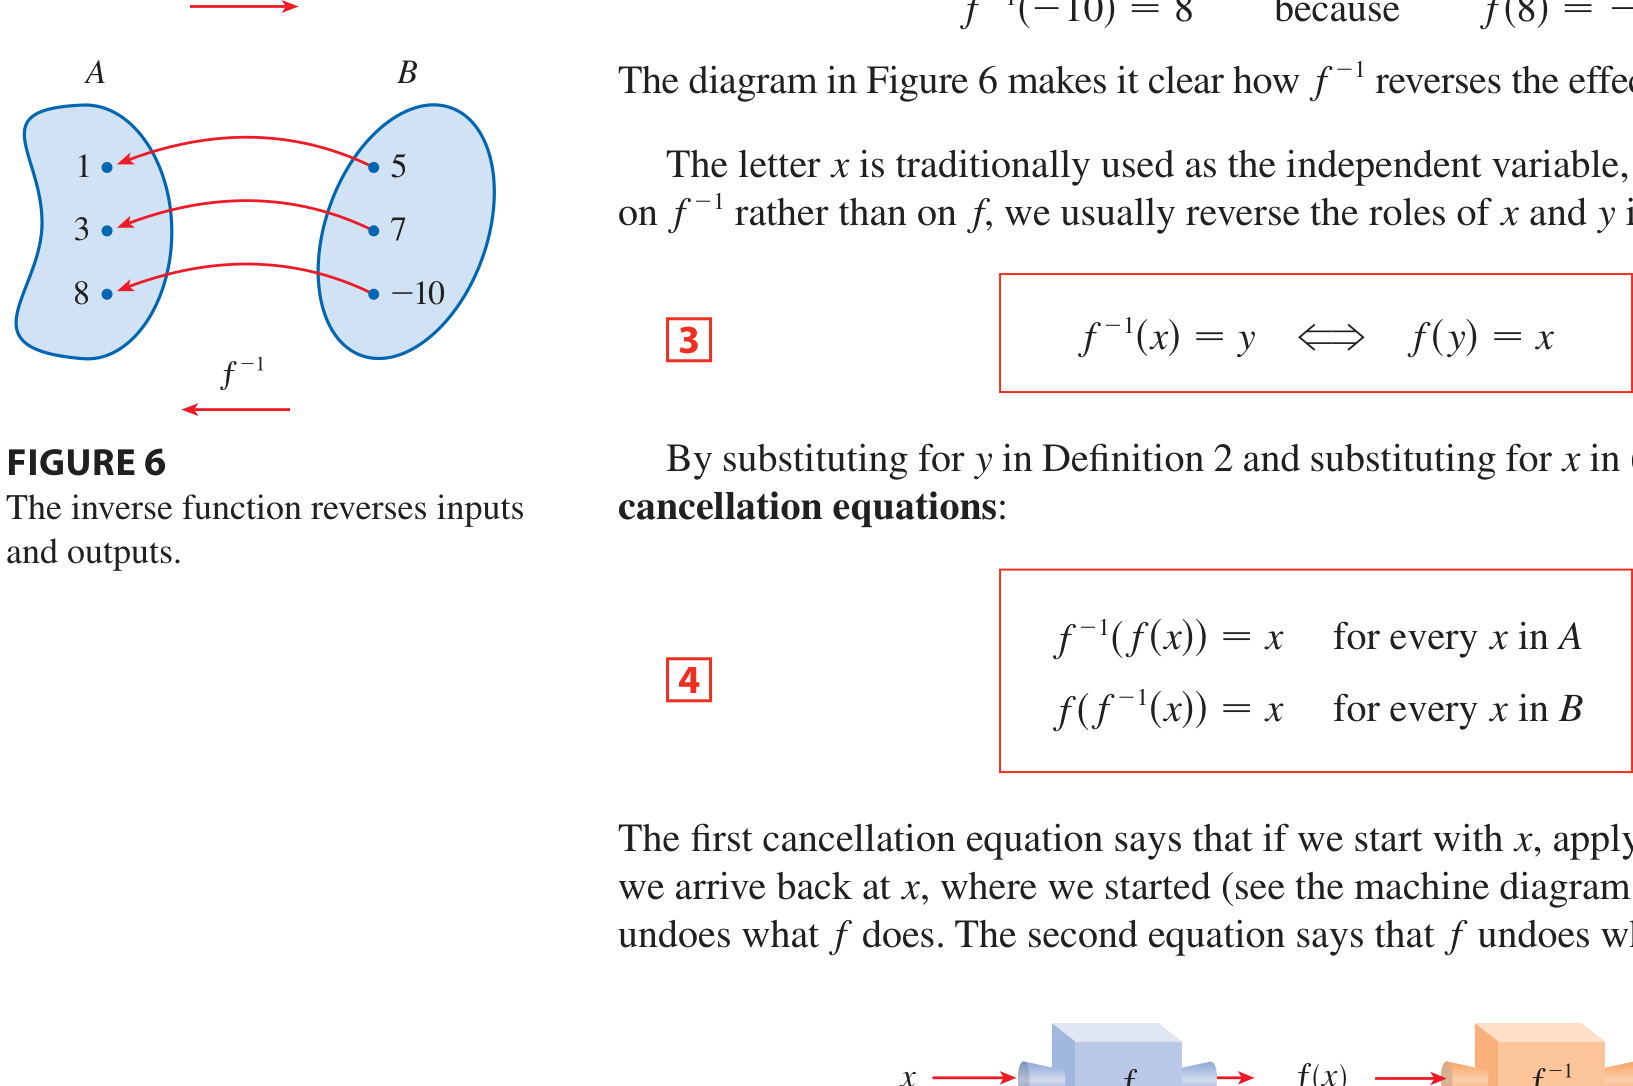
\includegraphics[width=0.92\linewidth]{images/p0091_fig7.png}
    \vspace{3pt}

    \textbf{\textsf{HÌNH 7}}
\end{minipage}%
\hfill
\begin{minipage}[t]{0.708\textwidth}
    \fontsize{9.3pt}{13.2pt}\selectfont
    \vspace*{0pt}
    \noindent
    \textbf{\textsf{\color{stewartcyan}VÍ DỤ 3}}\quad Nếu $f$ là một hàm đơn ánh thỏa mãn $f(1) = 5$, $f(3) = 7$ và $f(8) = -10$, hãy tìm $f^{-1}(7)$, $f^{-1}(5)$ và $f^{-1}(-10)$.

    \vspace{4pt}
    \noindent
    \textbf{\textsf{\color{stewartcyan}LỜI GIẢI}}\quad Từ định nghĩa của $f^{-1}$, ta có
    \begin{align*}
        f^{-1}(7) &= 3 \quad \text{vì} \quad f(3) = 7 \\
        f^{-1}(5) &= 1 \quad \text{vì} \quad f(1) = 5 \\
        f^{-1}(-10) &= 8 \quad \text{vì} \quad f(8) = -10
    \end{align*}
    Sơ đồ ở Hình~6 làm sáng tỏ cách thức $f^{-1}$ đảo ngược tác động của $f$ trong trường hợp này.\hfill{\color{stewartcyan}$\blacksquare$}

    \vspace{6pt}
    Theo truyền thống, chữ cái $x$ thường được dùng làm biến độc lập, vì vậy khi chúng ta tập trung vào $f^{-1}$ thay vì $f$, ta thường đảo ngược vai trò của $x$ và $y$ trong Định nghĩa~2 và viết

    \vspace{4pt}
    \begin{center}
    \begin{minipage}{0.95\linewidth}
      \makebox[0pt][l]{\tikz[baseline=-0.6ex]{\node[draw=stewartred, line width=0.8pt, inner sep=2.5pt, font=\small\bfseries\color{stewartred}] {3};}}%
      \centering
      \tikz[baseline=-0.6ex]{\node[draw=stewartred, line width=0.8pt, inner xsep=28pt, inner ysep=7pt] {$\displaystyle f^{-1}(x) = y \iff f(y) = x$};}
    \end{minipage}
    \end{center}

    \vspace{4pt}
    Bằng cách thay cho $y$ trong Định nghĩa~2 và thay cho $x$ trong (3), ta nhận được các \textbf{phương trình triệt tiêu} sau:

    \vspace{4pt}
    \begin{center}
    \begin{minipage}{0.95\linewidth}
      \makebox[0pt][l]{\tikz[baseline=-0.6ex]{\node[draw=stewartred, line width=0.8pt, inner sep=2.5pt, font=\small\bfseries\color{stewartred}] {4};}}%
      \centering
      \tikz[baseline=-0.6ex]{\node[draw=stewartred, line width=0.8pt, inner xsep=20pt, inner ysep=7pt] {$\displaystyle
      \begin{aligned}
          f^{-1}(f(x)) &= x \quad \text{với mọi } x \text{ trong } A \\
          f(f^{-1}(x)) &= x \quad \text{với mọi } x \text{ trong } B
      \end{aligned}
      $};}
    \end{minipage}
    \end{center}

    \vspace{4pt}
    Phương trình triệt tiêu thứ nhất nói rằng nếu ta bắt đầu với $x$, áp dụng hàm $f$, rồi sau đó áp dụng hàm $f^{-1}$, ta sẽ quay trở lại đúng giá trị $x$ ban đầu (xem sơ đồ máy ở Hình~7). Do đó, $f^{-1}$ đảo ngược những gì $f$ thực hiện. Phương trình thứ hai nói rằng $f$ đảo ngược những gì $f^{-1}$ thực hiện.

    \vspace{6pt}
    Chẳng hạn, nếu $f(x) = x^3$, thì $f^{-1}(x) = x^{1/3}$ và do đó các phương trình triệt tiêu trở thành
    \begin{align*}
        f^{-1}(f(x)) &= (x^3)^{1/3} = x \\
        f(f^{-1}(x)) &= (x^{1/3})^3 = x
    \end{align*}
    Các phương trình này chỉ đơn giản nói rằng hàm lũy thừa bậc ba và hàm căn bậc ba triệt tiêu lẫn nhau khi được áp dụng kế tiếp nhau.

    \vspace{6pt}
    Bây giờ chúng ta hãy xem cách tìm các hàm ngược. Nếu ta có một hàm số $y = f(x)$ và có thể giải phương trình này để tìm $x$ theo $y$, thì theo Định nghĩa~2, ta phải có $x = f^{-1}(y)$. Nếu muốn dùng ký hiệu biến độc lập là $x$, khi đó ta hoán đổi vị trí của $x$ và $y$ để nhận được phương trình $y = f^{-1}(x)$.

    \vspace{6pt}
    \begin{tcolorbox}[colframe=stewartred, colback=white, boxrule=0.8pt, arc=0mm, left=10pt, right=10pt, top=8pt, bottom=8pt]
    \noindent
    \tikz[baseline=-0.6ex]{\node[draw=stewartred, line width=0.8pt, inner sep=2.5pt, font=\small\bfseries\color{stewartred}] {5};}%
    \hspace{6pt}\textbf{\textsf{\color{stewartred}Cách tìm hàm ngược của một hàm đơn ánh $f$}}\\[6pt]
    \textbf{\textsf{BƯỚC 1}}\quad Viết $y = f(x)$.\\[4pt]
    \textbf{\textsf{BƯỚC 2}}\quad Giải phương trình này để tìm $x$ theo $y$ (nếu có thể).\\[4pt]
    \textbf{\textsf{BƯỚC 3}}\quad Để biểu diễn $f^{-1}$ như một hàm theo biến $x$, ta hoán đổi $x$ và $y$.\\
    \phantom{\textbf{\textsf{BƯỚC 3}}\quad }Phương trình kết quả nhận được là $y = f^{-1}(x)$.
    \end{tcolorbox}
\end{minipage}